% ===================================================
% CHAPITRE 11 — MONTAULIEU
% Pages imprimées 57-61 — vues 60-64
% ===================================================
\chapter{Montaulieu}

% --- Page imprimée 57 — vue 60
Le Château de Montaulieu, construit au midi d'Ouroux, sur le plateau qui domine la vallée de la Grosne, n'était plus au siècle dernier qu'une ruine à laquelle on donne encore le nom de Château du Bois. Ce fief existait-il avant le commencement du XVII° siècle ? Ici encore, nous ne pouvons répondre que par des hypothèses mais il est probable qu'il a été érigé après le démembrement de celui de Nagu.

\begin{center}
    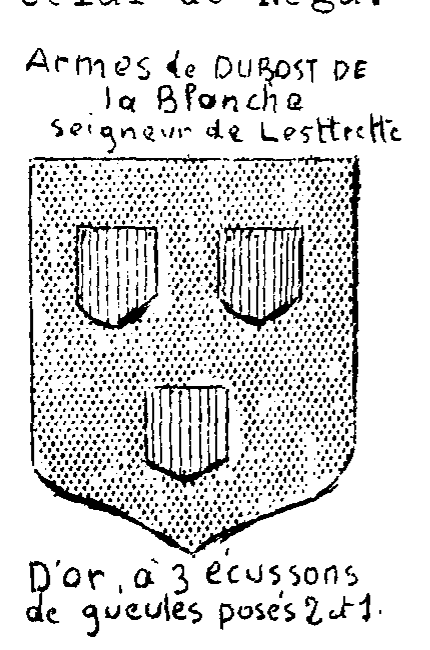
\includegraphics[width=0.20\textwidth]{Illustrations/illus-montaulieu-dubost.png}
\end{center}
Le premier possesseur de cette terre dont le nom nous est connu est Charles de la Blanche, sieur Dubost qui vivait en 1626, comme nous pouvons le constater dans un "acte d'eschange par lequel il remit à Jean Truchard une maison, cour et jardin situés à Chambuard".

L'histoire de nos contrées nous fournit peu de renseignements sur cette famille, nous éprouvons même quelque hésitation à en fixer le nom. Certains titres, en effet, et en particulier un acte de fondation faite à la Chapelle de St-Antoine, portent : "Charles de la Blanche, sieur Dubost" ; d'autres "Dubost, seigneur de la Blanche".

Le nom de la famille était-il Dubost ? Cette solution nous paraît préférable. À Saint-Nizier-d'Azergues existait un fief appelé Du Bost et possédé par les Seigneurs du même nom. Les derniers possesseurs du fief de Lettrete à Lestra portaient le nom de Du Bost.

% --- Page imprimée 58 — vue 61
de la Blanche et il paraît vraisemblable qu'ils appartenaient à la même famille que celle de Montaulieu.

Le nom de Dubost s'est d'ailleurs conservé jusqu'à nos jours et l'on ne peut donner d'autre étymologie à la désignation actuelle du Château-du-Bois que celle du nom latin De Bosco que l'on traduisit, comme nous l'avons vu, par Dubost ou Du Bois. Dans les titres officiels, le fief conserva le nom de son possesseur primitif malgré les changements qui se produisirent plus tard.

Cette confusion de nom ne doit pas nous surprendre. La famille De Bosco eut pendant plusieurs siècles, dans nos provinces, un grand nombre de représentants. De 1300 à 1306 Guillaume De Bosco ; De 1306 à 1320, Jean De Bosco sont abbés de Saint-Rigaud. Dans le même siècle, l'un d'eux est veneur du sire de Beaujeu qui lui donne le fief de Pesseley, paroisse de St-Symphorien-de-Lay. Nous avons trouvé un De Bosco venant se fixer comme notaire à Ouroux au siècle suivant. Plusieurs fondations de messes furent faites par eux dans l'église de Beaujeu. Rien d'étonnant que le nom de Dubost ait fait place, dans le langage usuel et par suite dans les actes peu importants à celui des fiefs que possédait cette famille, afin d'établir une distinction nécessaire entre ses divers membres.

Charles Dubost, le premier dont le nom soit parvenu jusqu'à nous naquit vers la fin du XVIe siècle et épousa le 3 Novembre 1614, Huguette Testenoire, fille d'Étienne Testenoire et de Guillemette de Noblet ; elle appartenait, par son père, à la branche des Testenoire de Bacot.

Veuve en 1646, nous la voyons faire une donation en faveur de Gabriel Dubost son fils, écuyer et capitaine au régiment d'Auvergne

Gabriel Dubost, seigneur de la Blanche, la Tulle, Montaulieu et autres places, d'après un état des revenus des gentilhommes de notre paroisse dressé en 1656, possédait dans notre paroisse six domaines son château de Montaulieu et un pré de réserve, le tout du revenu de 910 livres. Le "roolle des grandes tailles, taillon..etc ; " publié en 1674, mentionne sept domaines comme lui appartenant : cinq à la Combe du Thel, un au château Montagne et un à la Combe d'Aissard.

En 1664, il avait loué à Claude de Grosbois, bourgeois à St-Mamert et à Claude du Croux dict Beaux laboureur dudit lieu "la thuillière
% --- Page imprimée 59 — vue 62 (suite)
située proche le bourg d'Ouroux moyennant 3000 thuilles creuses, une botte chaux, le tour bien quy".

Nous retrouvons encore son nom cité en 1702; il payait à cette époque à Jean Hugues Duligier pour la rente Noble d'Ouroux appartenant à son Altesse Royale, Monsieur, la somme de 36.

Lui ou ses héritiers vendirent leur fief au commencement du siècle dernier à la famille de Fautrière.

Le 28 Décembre 1669 Gabriel Dubost, par un acte reçu Testenoire, notaire royal, fonda douze messes dans la Chapelle Saint-Antoine dont il devint le patron et qu'il choisit comme lieu de sa sépulture.

Famille de Fautrières

\begin{wrapfigure}{l}{0.42\textwidth}
    \vspace{-0.8\baselineskip}
    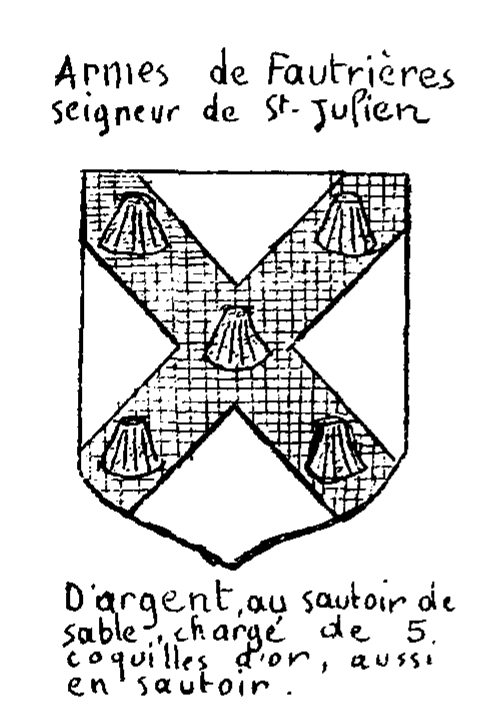
\includegraphics[width=0.39\textwidth]{Illustrations/illus-montaulieu-fautrieres.png}
\end{wrapfigure}

Cette famille, propriétaire du château de Corcheval, paroisse de Beaubéry dans la Saône et Loire, était très ancienne. Elle avait donné son nom à une localité appelée Fautrières, autrefois paroisse, réunie en 1823 à Palingues chef lieu de Canton.

D'après la généalogie complète que nous possédons, le premier dont le nom nous soit connu Antelme de Fautrières, vivait en 1060. La famille s'est éteinte en 1792 dans la personne de Jean Louis de Fautrières mort célibataire. Antelme fut l'aïeul, au 16° degré, en ligne directe de Claude de Fautrières qui naquit le 19 avril de l'année 1629. Ce dernier épousa le 4 Septembre 1656 Elisabeth de Chapon, fille unique de Jean de Chapon, sieur de la Bothière et Angélique de St-Julien, héritière du fief de même nom situé à St-Mamert.

Ce fut sans doute par suite de cette alliance qu'il devint propriétaire de plusieurs domaines situés sur la paroisse d'Ouroux. "L'estat des revenus" dont nous avons parlé plus haut atteste qu'il possédait trois domaines amodiés au prix de 600 livres. En 1674 il a quatre "grangiers": un au bourg, l'autre à la Combe, le troisième aux Pourchoux et le quatrième à la Combe d'Aissard, plus deux appentionnaires non nommés. Nous ne savons pour quel motif on a
% --- Page imprimée 60 — vue 63 (suite)
passé sous silence le mas Dagain qui lui appartenait également à cette époque.

D'après son codicille du 9 Octobre 1674, il eut d'Elisabeth de Chapon treize enfants; les sept premiers furent tués pendant les guerres de Louis XIV. Le huitième, Claude Marie, entra à son tour dans l'armée. Il épousa Elisabeth de Perrault dont il eut un fils: Michel de Fautrières, lieutenant du roi au bailliage de Charollais. Ce dernier épousa, le 4 Septembre 1724, Laure Anne de la Tour et Taxis. Ayant eu une épaule et une jambe cassées d'une chute de cheval, il fut forcé de quitter le service militaire. Il eut plusieurs enfants.

Hélène Esprit, deuxième enfant de Michel de Fautrières épousa le 17 Février 1747 Jean François de Laurencin, Comte de Laurencin, seigneur d'Avenas, le Sausey, auquel elle apporta en dot la terre de Montolieu.

Famille de Laurencin

\begin{wrapfigure}{l}{0.42\textwidth}
    \vspace{-0.8\baselineskip}
    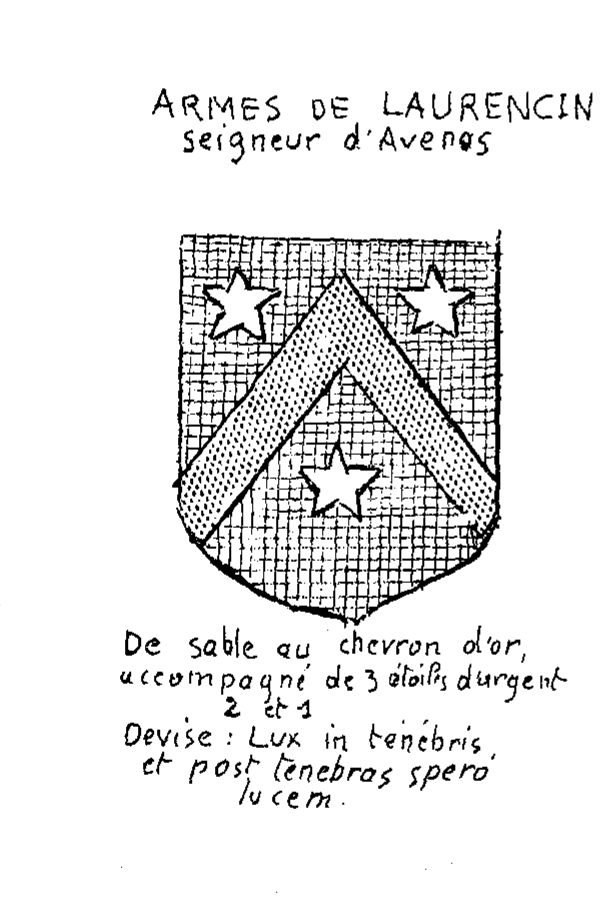
\includegraphics[width=0.39\textwidth]{Illustrations/illus-montaulieu-laurencin.png}
\end{wrapfigure}

Jean François de Laurencin, Comte d'Avenas, capitaine au régiment de Navarre.. appartenait à la branche des seigneurs de Beaufort en Comté par son aïeul Raimond de Laurencin.

Il est un acte passé quelques jours avant le mariage d'Hélène Esprit et que nous ne saurions passer sous silence ; nous n'en citerons que les dispositions principales.

"Haut et puissant seigneur Messire Michel, Comte de Fautrières, chevalier seigneur de Corcheval, Montaulieu, etc... lieutenant du roi de la province du Charollais, habitant son château de Corcheval, donne en amodiage à Honoré Jambon de Braille, fermier de Montaulieu, tout ce qu'il tient moyennant 100 " par an. Le Comte se réserve tous les bois et taillis, sauf le tiers du bois de Montlong, une chambre à cheminée au château pour loger le garde des bois et deux petits jardins du côté du soir. De plus, lorsque ledit Seigneur ou homme de sa part irait audit lieu pour recevoir ses rentes

% --- Page imprimée 61 — vue 64
Honoré Jambon serait tenu de loger au château et de nourrir ses chevaux, pendant trois jours". Cet acte fut passé à Beaubéry le 13 Février.

La même année un ouragan causa au château des dégâts considérables ; le couvert fut transporté tout entier de l'autre côté de la cour, dans la terre qui se trouve au nord-est de cette cour.

Tel était Montaulieu lorsque Hélène de Fautrières l'apporta en dot à la famille de Laurencin.

Jean François de Laurencin eut un fils nommé Philippe Laure, qui se maria avec Claudine Lafont de la Roole dont il eut une fille : Aimée.

Aimée de Laurencin qui fut mariée à Gérard Magdeleine Grégoire de Faultrière de Montaulieu, l'un des descendants de la famille de Fautrières qui avait possédé le fief de Montaulieu dont il avait gardé le nom. Il mourut sans postérité.

Aimée mourut elle-même à Paris le 13 Avril 1832.

Sa mère Claudine Lafont, qui vivait encore et avait épousé en secondes noces Gaspard Darod hérita de la moitié de la succession de sa fille. Henri François Jérôme, Prudence Mélanie et Gaspérine Désirée cousins paternels du sixième degré d'Aimée Emilie de Laurencin héritèrent de l'autre moitié.

Les revenus de Montaulieu étaient, à cette époque, de 1.086,50 au capital de 22.750 francs plus 12 poulets, 8 chapons, 18 mesures d'avoine, 1 mesure de froment et 4 charrois.

D'après les pièces du procès qui eut lieu entre Henri, Prudence et Gaspérine, les Laurencin avaient fondé un lit à l'hôpital de Beaujeu.

Le château de Montaulieu n'a jamais été fortifié. D'après le plan cadastral de la paroisse d'Ouroux dressé après 1747 et dont le 9° feuillet nous a été conservé, la Cour précédée d'une "place" triangulaire dans laquelle on débouchait par une assez belle avenue était bornée au midi par un vaste bâtiment en forme de parallélogramme qui existe encore. Deux tours donnaient à cette modeste construction une apparence seigneuriale.
